\chapter{从理论推导和本质参透的角度理解VAE}
% \label{sec:second}

\section{AE(Autoencoder)}
自编码器的基本结构如图所示,由一个编码器(Encoder),解码器(Decoder),两个之间是一个瓶颈(潜在空间)。
\subsection{主要的运行逻辑}
如图\ref{fig:ae}所示,
编码器把数据分布映射到潜在空间中,然后通过解码器把潜在空间中的分布映射回真实数据所在的空间中,以达到提取数据特征(编码器)和数据生成(解码器)的目的。
\begin{figure}[htbp]
    \centering
    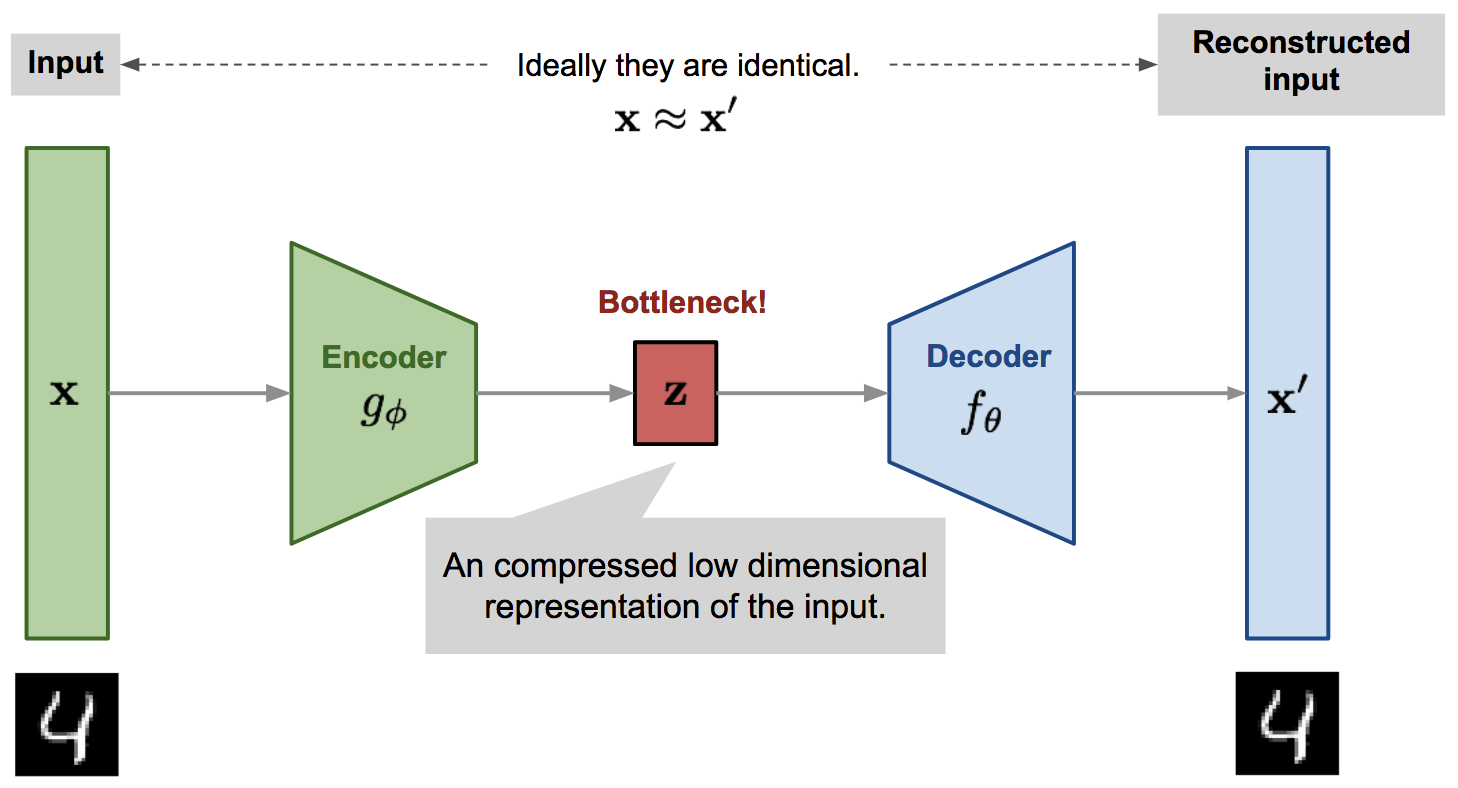
\includegraphics[width=\textwidth]{figures/chapter2/ae.png}
    \caption{自编码器的基本结构}
    \label{fig:ae}
\end{figure}

\subsection{如何理解图像分布?}
\textbf{先说说数据分布}

例如对于骰子而言,投到1~6的概率都是$\frac{1}{6}$,因此投骰子的这个事件的数据分布就是左图

\textbf{再说图像分布}

同样的,这时候我们把图片中成万上亿个像素所有的无数种可能性投影到二维的x轴上,这时候对于“图片为猫”这个事件来说,像素组成长得越像猫,其概率就越大,因此分布如\ref{fig:data_distribution}右图。

\begin{figure}[htbp]
    \centering
    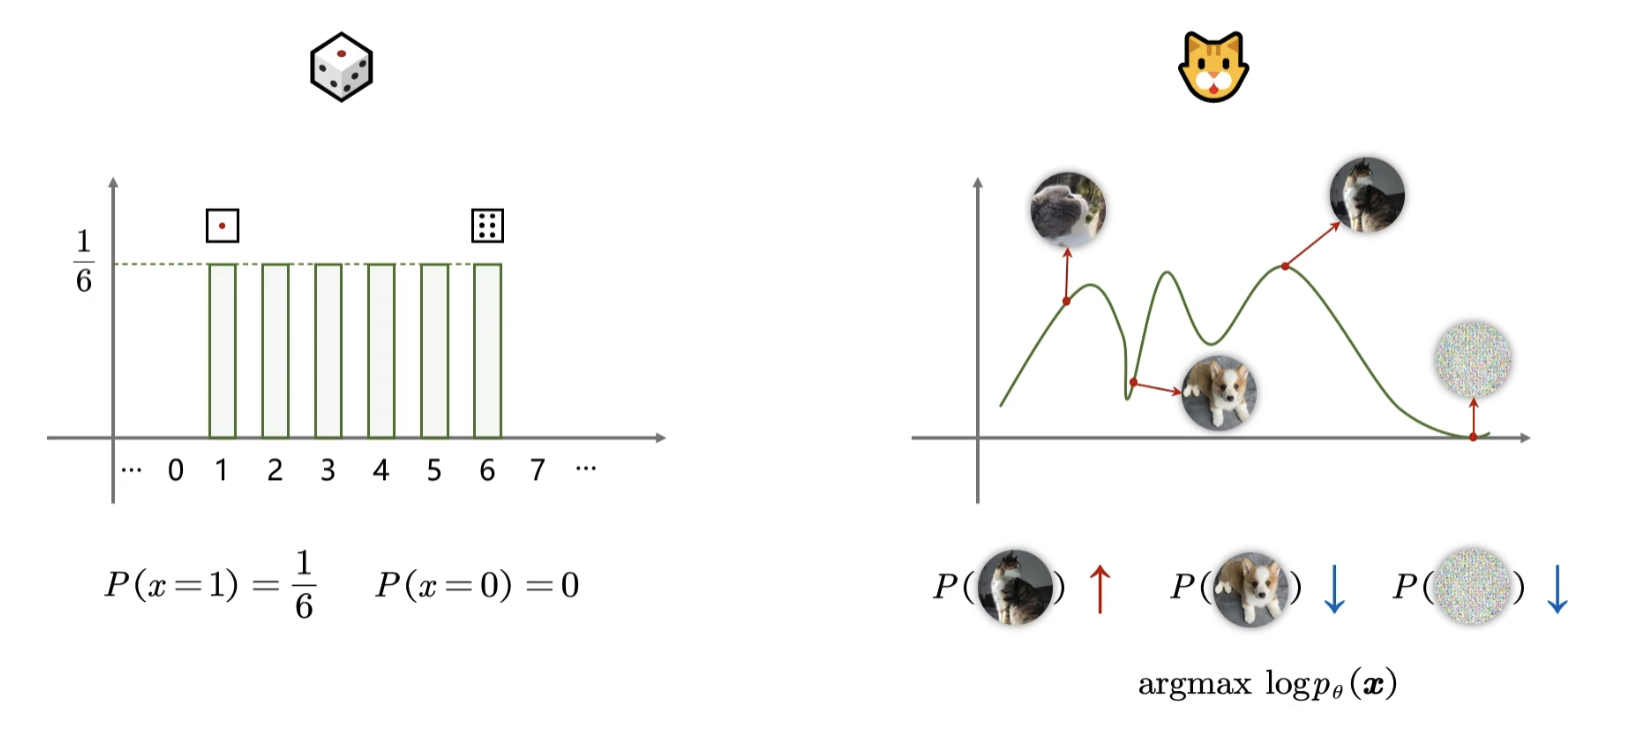
\includegraphics[width=\textwidth]{figures/chapter2/dis.png}
    \caption{数据分布}
    \label{fig:data_distribution}
\end{figure}

\subsection{缺陷?}
这种设计有什么缺陷呢? \newline
一般的潜在空间是一个n维的向量,这样的话会造成两个问题:
\begin{enumerate}
    \item 维度的选择很苛刻 
        \begin{itemize}
            \item 如果维度太低,模型可能无法捕捉足够的特征,欠拟合
            \item 如果维度过高,模型容易记住不重要的信息,过拟合
        \end{itemize}
    \item 模型的泛化能力差(硬伤) \newline
    原因是这种形式的隐空间特征值是离散的,从实验上看,离散值的特征无法保证在两个有意义的值之间的采样的数据同样有意义。
    \begin{quote}
        \textbf{举个例子}
        例如向量(0,...)的0表示图片中的人不笑,(2,...)中的2表示笑,那么当我们在生成的时候取(1,...)进行解码的时候未必得到一个介于不笑和笑之间的状态,很可能没有意义。
        同样的例子可见图\ref{fig:ae_example}。
    \end{quote}
    \begin{figure}[htbp]
        \centering
        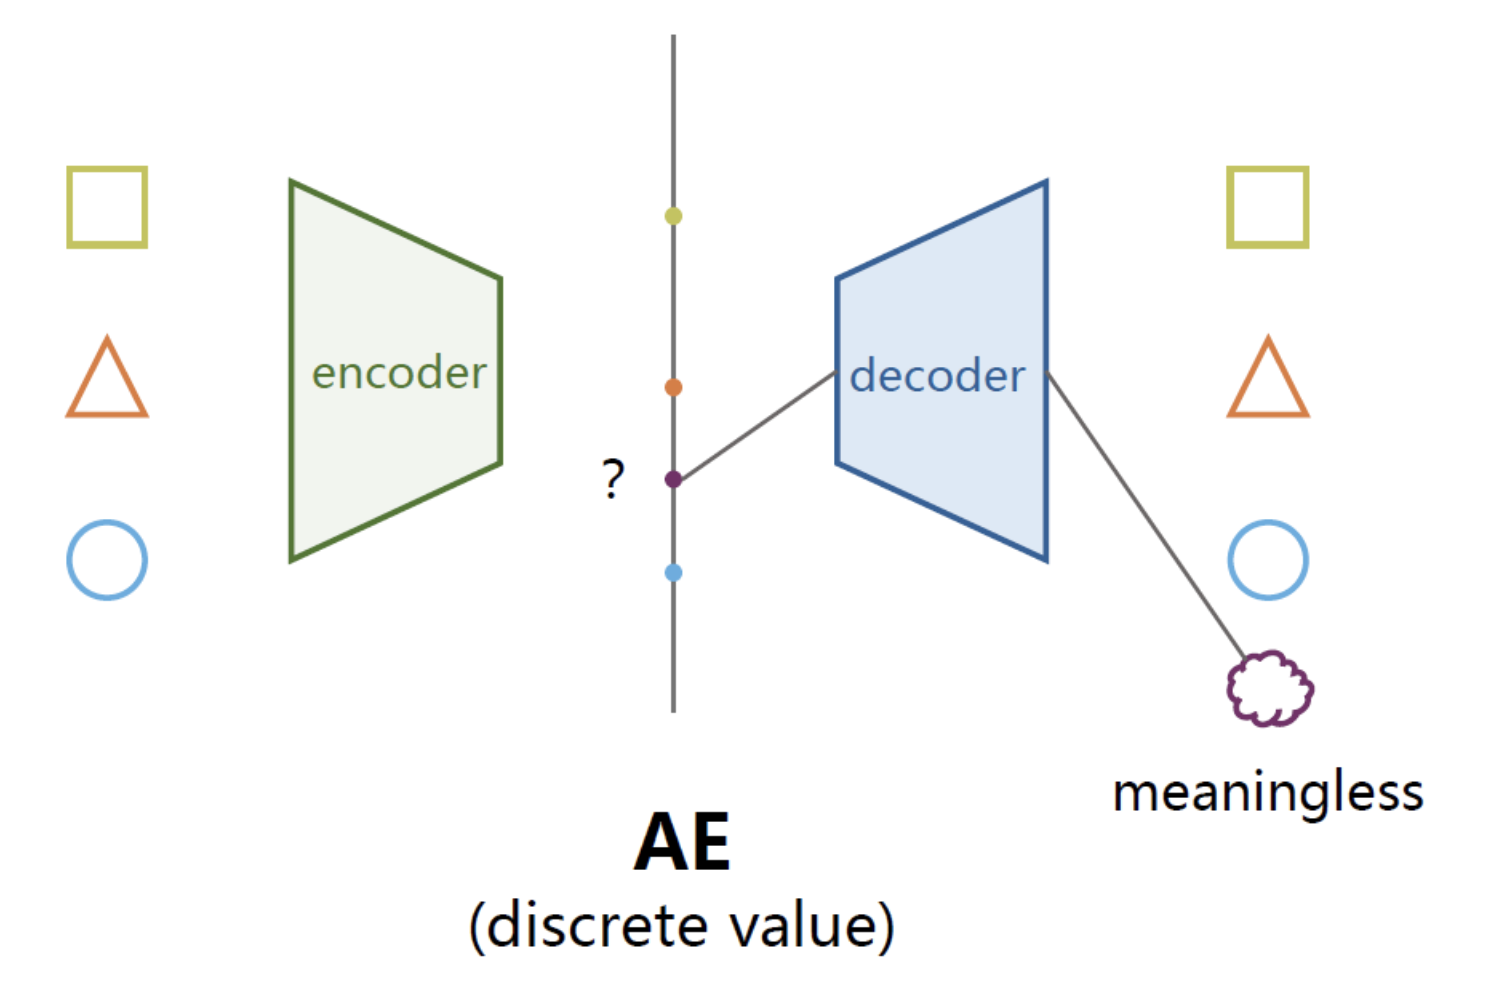
\includegraphics[width=0.8\textwidth]{figures/chapter2/aeeee.png}
        \caption{自编码器生成示例}
        \label{fig:ae_example}
    \end{figure}
\end{enumerate}

\section{VAE(Variational Autoencoder)}
变分自编码器的实现逻辑就是着重解决上述的第二个硬伤缺陷,既然离散的值没有办法保证平滑,那就把每个特征都记作一个分布,分布的移动之间就是连续的,如图\ref{fig:vae}。

\begin{figure}[htbp]
    \centering
    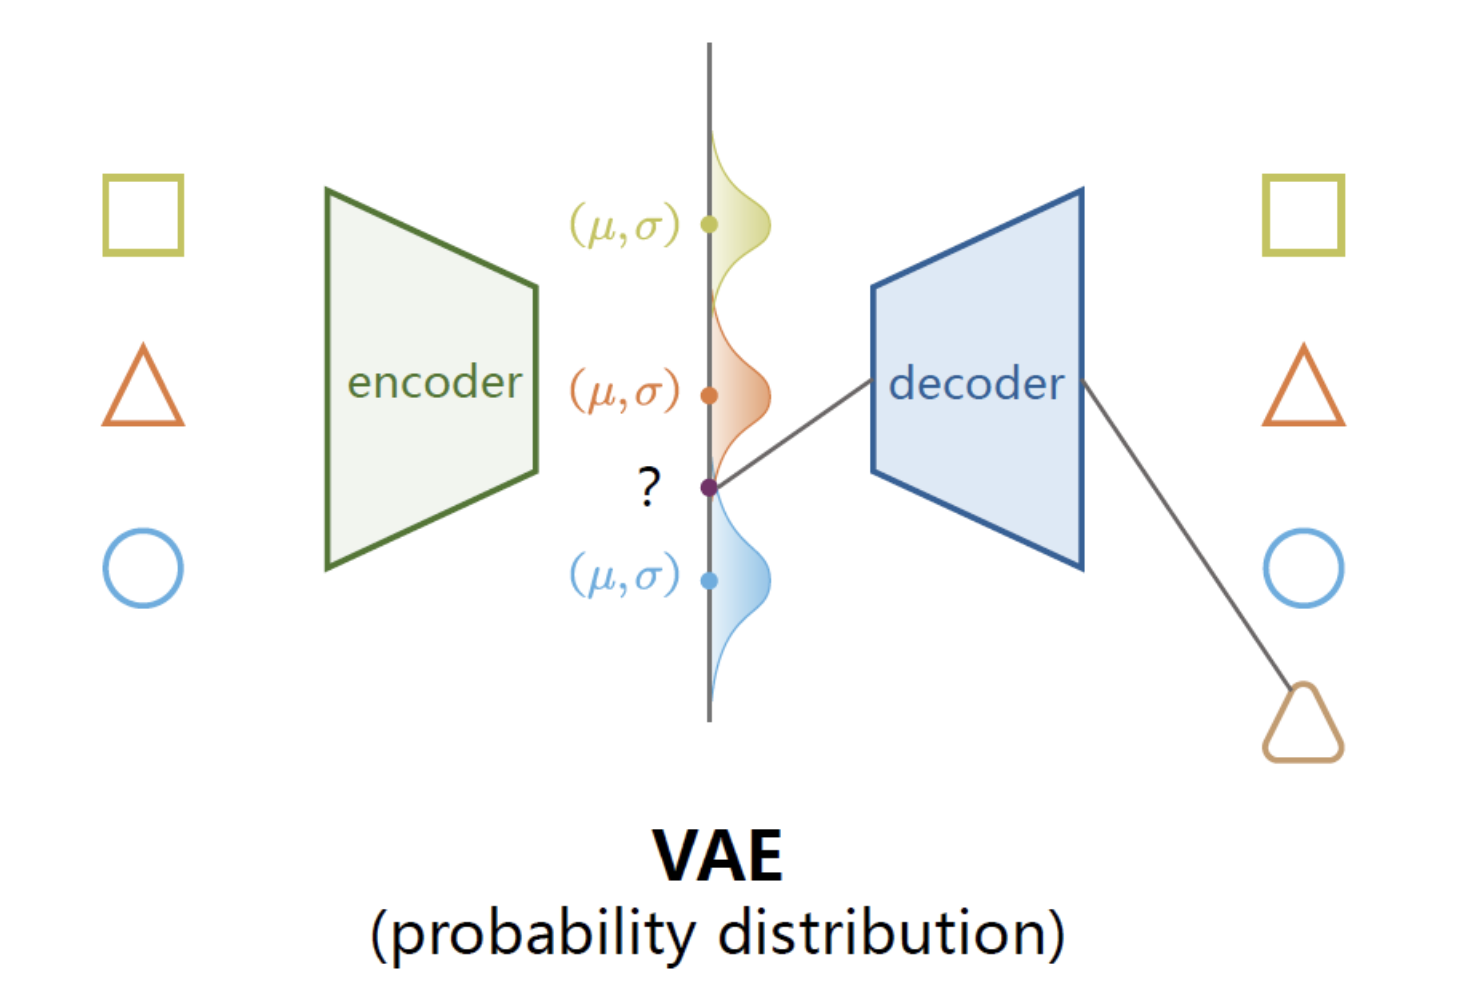
\includegraphics[width=0.8\textwidth]{figures/chapter2/vae.png}
    \caption{变分自编码器的基本结构}
    \label{fig:vae}
\end{figure}
\begin{quotation}
    “A variational autoencoder can be defined as being an autoencoder whose training is regularized to avoid overfitting and ensure that the latent space has good properties that enable generative process.”
\end{quotation}
VAE的出发点和AE的是一样的,希望构建一个从隐变量Z生成目标数据X的模型

\subsection{基本假设}
\textbf{假设隐变量Z的分布是标准正态分布} \newline
这个假设是不显然的,需要一定的解释和证明为什么可以做此假设

\textbf{高斯混合模型\&中心极限定理}\newline
从贝叶斯统计的角度来看,选择正态分布作为先验时基于中心极限定理
\begin{quotation}
    “中心极限定理指出,在一定条件下,大量独立随机变量的和近似于正态分布”
\end{quotation}
又有高斯混合模型
\begin{quotation}
    “假设所有的数据点都是从有限数量的高斯分布中生成的。每个高斯分布称为一个“分量”,而整个数据集可以看作是这些分量的加权组合。”
\end{quotation}
类似泰勒展开,一切分布都可以由若干个均值方差各异的高斯分布叠加而来,如图\ref{fig:gmm},
这可以表明高斯分布对于任一现实世界数据分布来说是“图灵完备”的,
但是这解释不了为什么标准高斯分布有效。
\begin{figure}[htbp]
    \centering
    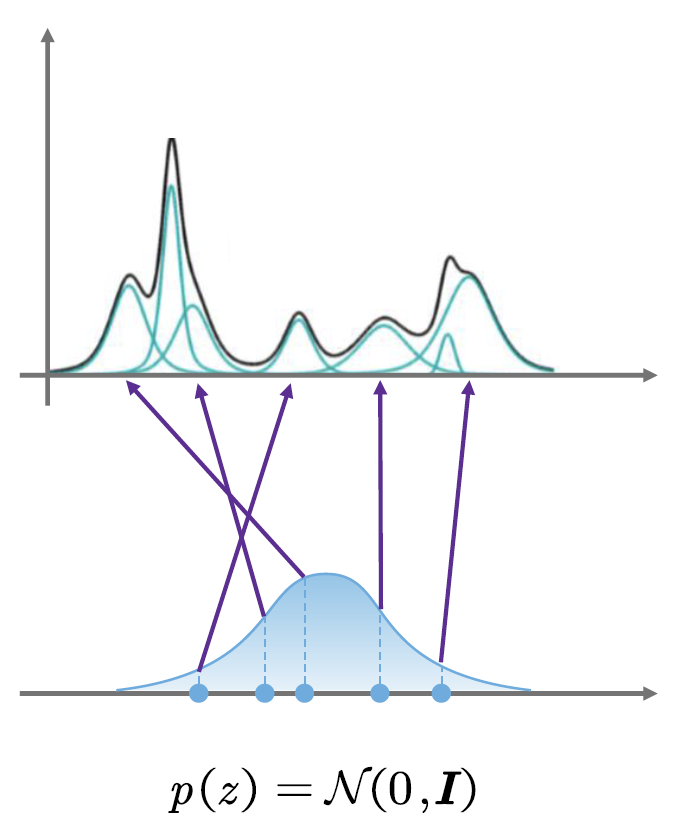
\includegraphics[width=0.5\textwidth]{figures/chapter2/gmm.png}
    \caption{高斯混合模型}
    \label{fig:gmm}
\end{figure}

\textbf{为什么标准高斯分布有效?}\newline
\label{sec:why_normal_distribution}
高斯分布的密度函数为
\begin{equation}
    f(x) = \frac{1}{\sqrt{2\pi\sigma^2}}e^{-\frac{(x-\mu)^2}{2\sigma^2}}
\end{equation}
对于上图中分布的每一个点,其上的值都表示一个概率,但是我们知道\textbf{密度函数不表示概率,一段密度函数的积分才是概率}
我们对密度函数进行积分可以发现

\begin{align}
    &\frac{1}{\sqrt{2\pi\sigma^2}} \int \exp\left(-\frac{(x - \mu)^2}{2\sigma^2}\right)dx  \\
    =& \frac{1}{\sqrt{2\pi}} \int \exp\left(-\frac{(x - \mu)^2}{2\sigma^2}\right)d\left(\frac{x-\mu}{\sigma}\right)
\end{align}

得出的结论和概率论常识结论匹配:
\begin{enumerate}
    \item 对方差为$\sigma$的高斯分布采样,得到的结果从概率上看与标准高斯分布同一点的采样只是差了一个常数系数
    \item 而均值只是对应x轴的移动而已
\end{enumerate}

这两点都是可以由解码器实现,只需要在解码的时候对于每个特征的分布进行方差和均值的变化,然后通过前面的高斯混合模型对目标数据分布进行还原
\textbf{为何标准高斯分布?}\newline
\begin{enumerate}
    \item \textbf{简化运算};在后续需要进行KL散度的计算中,使用标准高斯分布的话,KL散度有一个\textbf{闭式解},大大简化了优化问题。
    \item \textbf{平滑性和连续性};高斯分布是平滑且连续的,有助于生成更加自然和平滑的数据脚本
    \item \textbf{无信息先验};选择标准高斯分布意味着我们对潜在空间没有先验知识,有利于模型的泛化,帮助避免过拟合
\end{enumerate}

\subsection{VAE基本结构}
VAE和AE不同的地方在于其改变了隐空间的结构和隐变量的表达形式
\textbf{VAE与AE的异同}\newline
其基本目的和AE相同
\begin{enumerate}
    \item 对于数据$X$,用encoder提取出图片特征,得到隐变量
    \item 通过decoder对隐变量进行还原得到$X'$
    \item 通过让$X'$接近$X$来训练模型
\end{enumerate}
其实现逻辑与AE不同
\begin{enumerate}
    \item Encoder在VAE中的作用是对于采样$X$,都得到一对均值和方差
    \item 然后从标准正态分布中采样出一个$Z$,使用\textbf{重参数化}的技巧把均值和方差放在$Z$上
\end{enumerate}
\begin{figure}[htbp]
    \centering
    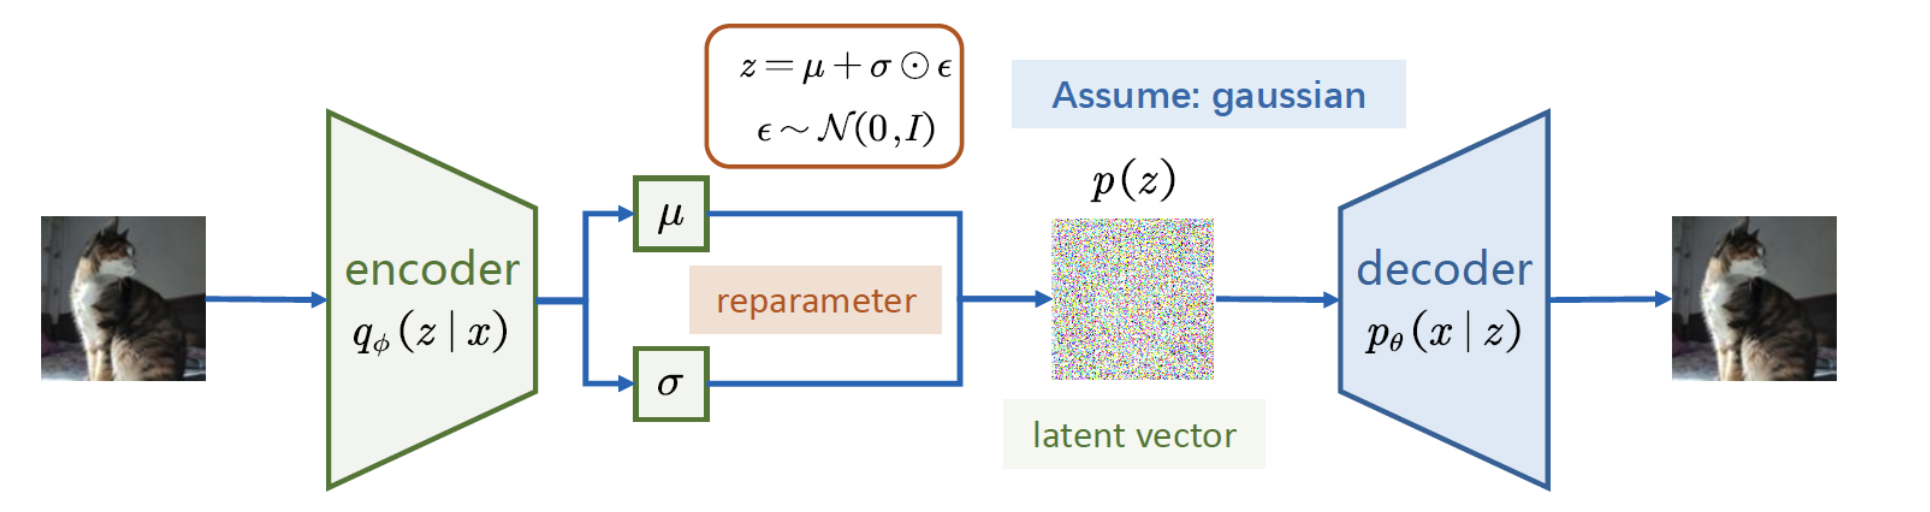
\includegraphics[width=\textwidth]{figures/chapter2/vaeee.png}
    \caption{VAE的结构}
    \label{fig:vae_structure}
\end{figure}

\textbf{重参数化技巧}\newline
\label{sec:reparameterization}
英文名叫做reparameterization trick,这里称其为重参数,
通过\ref{sec:why_normal_distribution}的结论我们可以把encoder得到的$\mu$和$\sigma$根据根据上图种重参数表达式放入隐变量中即可
\begin{quotation}
    从$N(\mu, \sigma^2)$中采样一个$Z$,相当于从$N(0, I)$中采样一个$\varepsilon$,然后让$Z=\mu+\varepsilon\times\sigma$。
\end{quotation}
这个结构是不好理解的,主要问题是有一个误区

\textbf{一个误区} \newline
\begin{figure}[htbp]
    \centering
    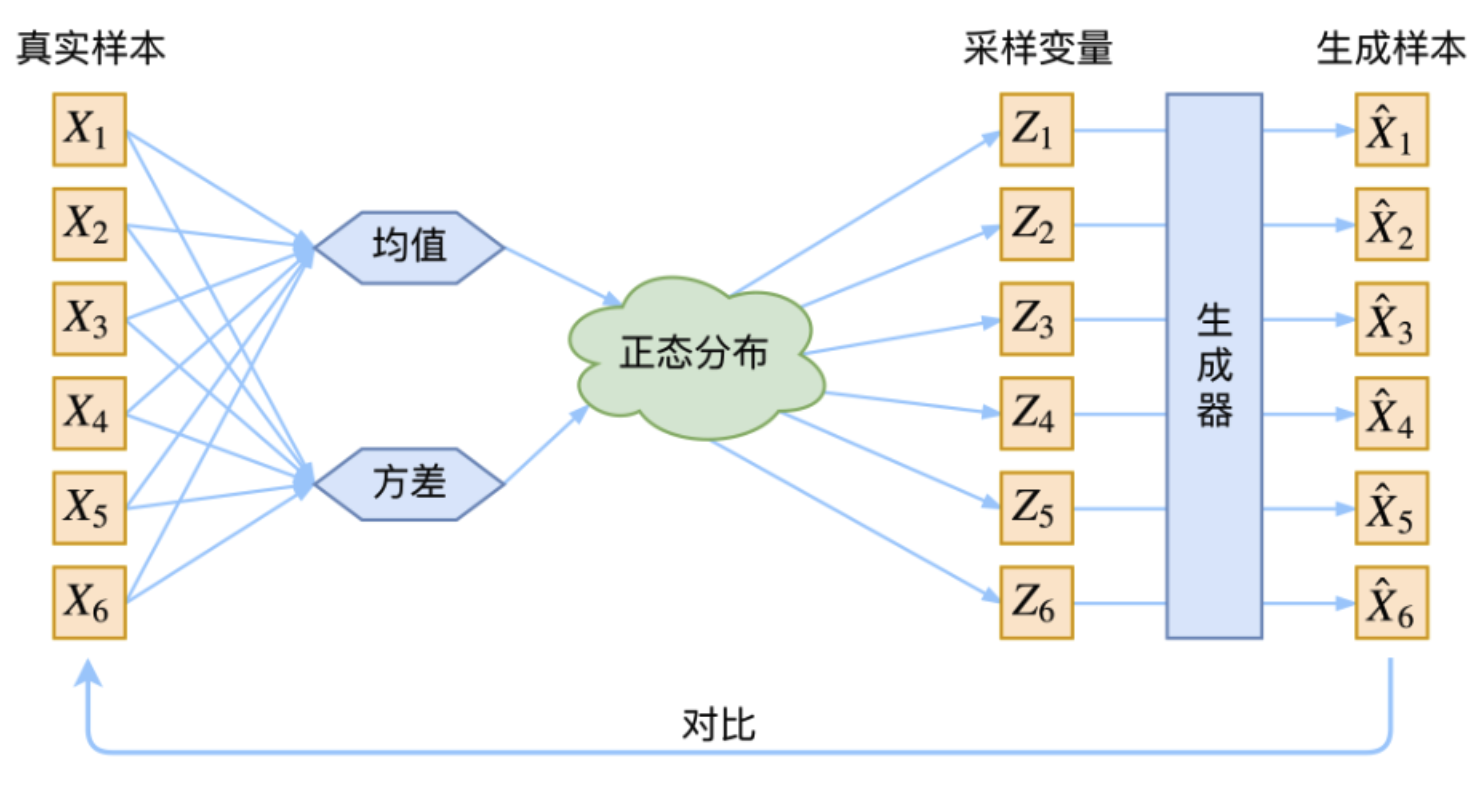
\includegraphics[width=0.8\textwidth]{figures/chapter2/vaeno.png}
    \caption{错误的VAE逻辑}
    \label{fig:vae_mistake}
\end{figure}
这样一个过程看起很对,但其实会让我们不禁想到这样一个问题: \newline
真实样本和生成样本真的是按下标一一对应的吗?\newline
\paragraph{错误逻辑}
如果按图\ref{fig:vae_mistake}的过程进行操作,那么从诸多的样本中取得均值方差,再放入正态分布中采样出同样数量个采样变量,这个过程中真实样本显然和采样变量并不是一一对应的,但是采样变量和生成样本是一一对应的,所以真实样本与生成样本根本不是一一对应的,也就无从对比了。
因此VAE真正的逻辑应当是,对于每个采样我们都得到一对均值方差,然后一一对应每个采样变量。
\begin{figure}[htbp]
    \centering
    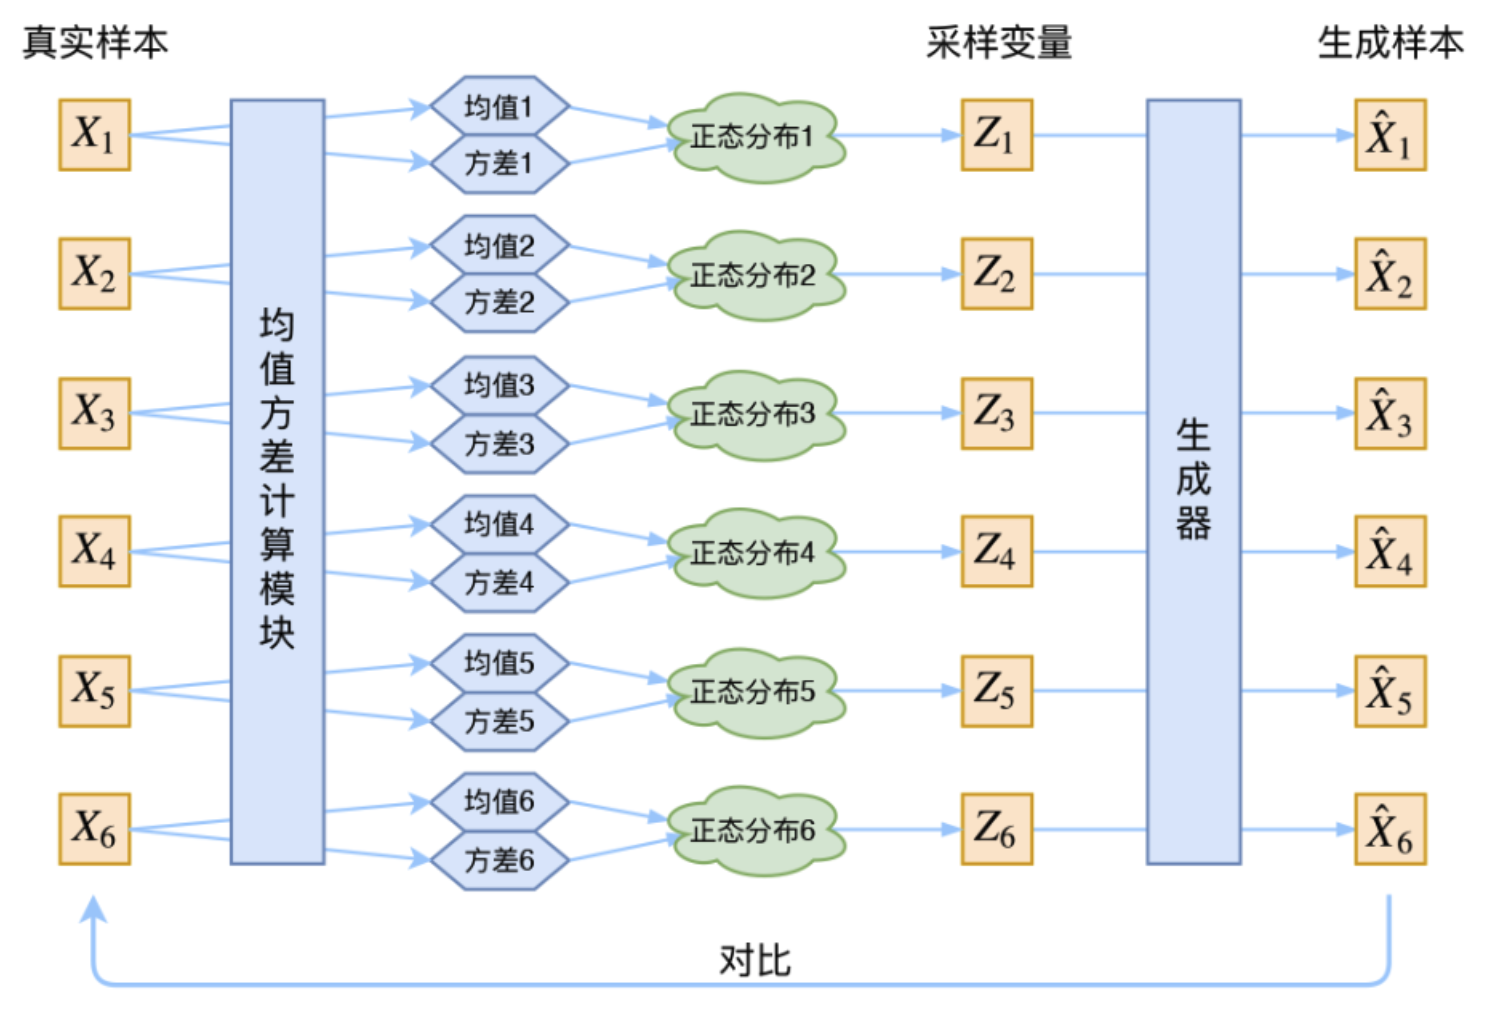
\includegraphics[width=0.8\textwidth]{figures/chapter2/vaeyes.png}
    \caption{正确的VAE逻辑}
    \label{fig:vae_correct}
\end{figure}
\paragraph{正确逻辑}
如图\ref{fig:vae_correct}所示,这里的样本可以看作是上面讨论的图像中的每一个像素。由于通常我们的隐空间的维度数是小于样本的,这样有助于提高效率,也有助于模型的泛化能力。
因此对于一张图片,我们会得到隐变量$Z$的维度数对均值方差,然后构建出隐变量,再通过生成器得到生成样本,这样可以使得生成样本和真实样本的每一个\textbf{隐变量维度表示的特征}是一一对应的。
解决了这个误区之后,还是\textbf{只是知其然,但是不知所以然} \newline
所以下面两种理解角度帮助理解。为了避免首先进行理论推导导致看不懂,无法与后续的本质参透进行对比理解的问题,我们先从本质开始,然后进行理论推导,最后再对比两者

\subsection{VAE本质是什么?}
\label{sec:vae_essence}
\paragraph{VAE的本质和GAN一样也是一组矛盾}
首先让我们focus目标数据和生成数据之间尽量接近这个过程,考虑这个过程会让模型向什么方向走
\begin{itemize}
    \item 这个过程会希望目标数据和生成数据差别越小越好
    \item 那么这样就会希望encoder给出的均值是图片本身的每种特征的均值,方差为0,这样隐变量会刚刚好得到真实图片本身的均匀分布,经过生成器,只需要对特征进行还原,就可以得到真实图片本身
    \item 这与我们需要模型是一个可泛化的生成器的初衷是相悖的。
\end{itemize}
所以我们设定了基本假设,要求隐变量$Z$是标准正态分布
\paragraph{如何让隐变量成为标准高斯分布?}
假设对于特征k,encoder给出均值和方差分为两个函数$f_{k1}$和$f_{k2}$,
为了保证方差非负,实际操作中encoder给出的通常是$log(\sigma^2)$。
首先\ref{sec:reparameterization}中提到$\varepsilon$从标准高斯分布中采样,其次就是我们希望encoder给出的均值尽量接近0,方差尽量接近1。\newline
我们大可以使用均方损失:\newline
考虑两个损失函数:  
\begin{itemize}
    \item 均方误差损失函数:
      \begin{equation}
        L_{\mu} = ||f_1(X_k)||^2
      \end{equation}
    \item 方差损失函数:
      \begin{equation}
        L_{\sigma^2} = ||f_2(X_k)||^2
      \end{equation}
\end{itemize}
但是这时候又会面临这两个损失的比例怎么选取的问题,选取的不好,生成的图像就会比较模糊。
因此作者直接算了一般正态分布和标准正态分布的KL散度$KL \left(N(\mu, \sigma^2) \Bigg\| N(0, I)\right)$。 \newline
这个loss是有闭式解的,可以得到
\begin{equation}
    KL \left(N(\mu, \sigma^2) \Bigg\| N(0, I)\right) = \frac{1}{2} \sum_{i=1}^{d} \left(\mu_i^2 + \sigma_i^2- 1 - \log(\sigma_i^2)\right)
\end{equation}
显然,这里的loss也可以分成两个部分理解:
\begin{align}
    L_{\mu,\sigma^2} &= L_{\mu} + L_{\sigma^2} \\
    L_{\mu} &= \frac{1}{2} \sum_{i=1}^{d} \mu_i^2 = \frac{1}{2} ||f_1(X_k)||^2 \\
    L_{\sigma^2} &= \frac{1}{2} \sum_{i=1}^{d} \left( \sigma_i^2 - 1 - \log(\sigma_i^2) \right)
\end{align}
这样就直观的多。
\begin{quotation}
    对于上述解的推导超出了本书的研究范围,感兴趣的读者可以自行推导。
\end{quotation}
然后反过来我们再focus隐变量尽量靠近标准正态分布这个过程。\newline
这个过程希望均值越接近0越好,方差越接近1越好
\paragraph{这与上面第一个损失是矛盾的!}
这个过程可以理解为两个loss之间的对抗(有点GAN的味道)。
$X$和$\hat{X}$靠近的Loss希望方差接近0,而KL散度表示的Loss希望方差(强度)接近1,均值接近0。
所以,VAE跟GAN一样,内部其实是包含了一个对抗的过程,只不过它们两者是混合起来,共同进化的。具体如图\ref{fig:vae_adversarial}。
\begin{figure}[htbp]
    \centering
    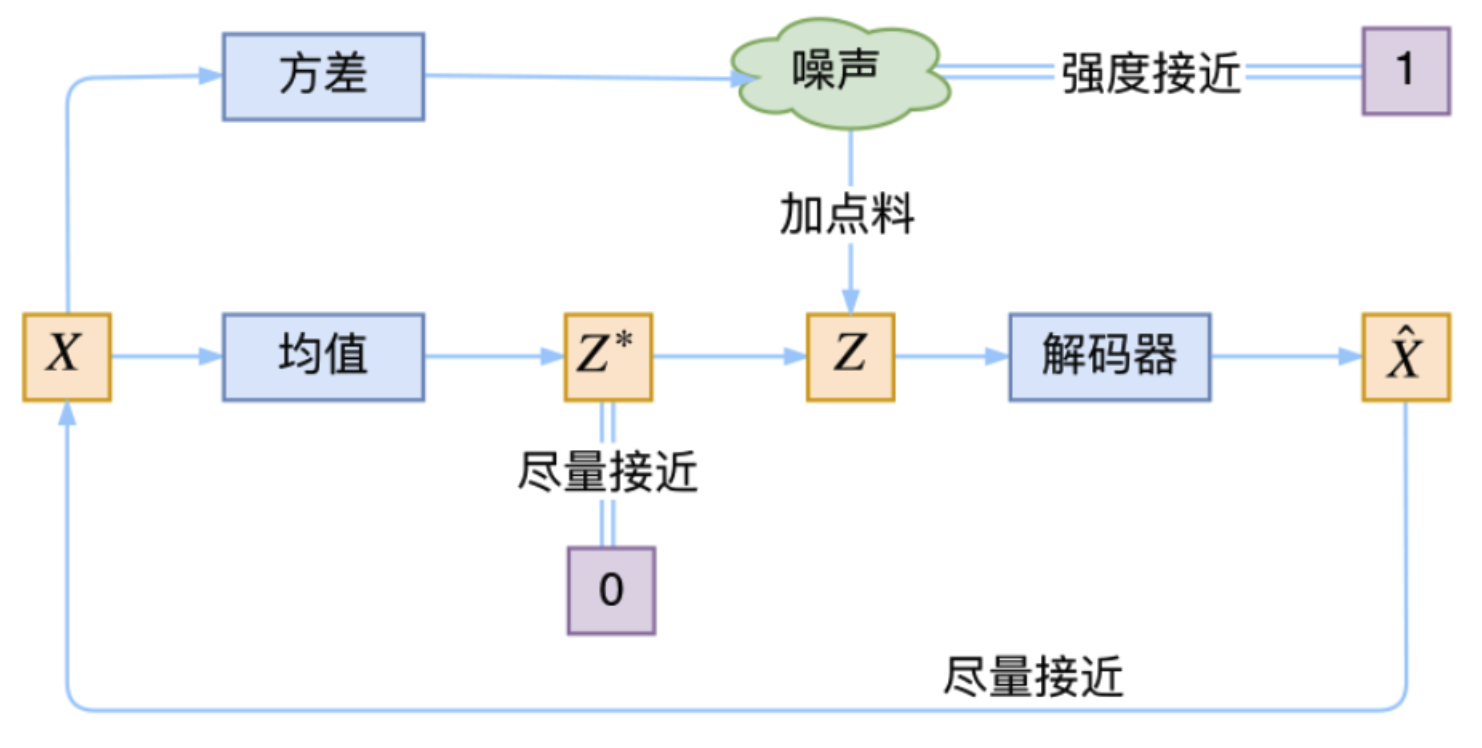
\includegraphics[width=\textwidth]{figures/chapter2/normalvae.png}
    \caption{VAE的对抗过程}
    \label{fig:vae_adversarial}
\end{figure}
当然这也给了我们控制生成的思路:\newline
只需要对于不同的类别控制不同的均值就可以实现。
\begin{figure}[htbp]
    \centering
    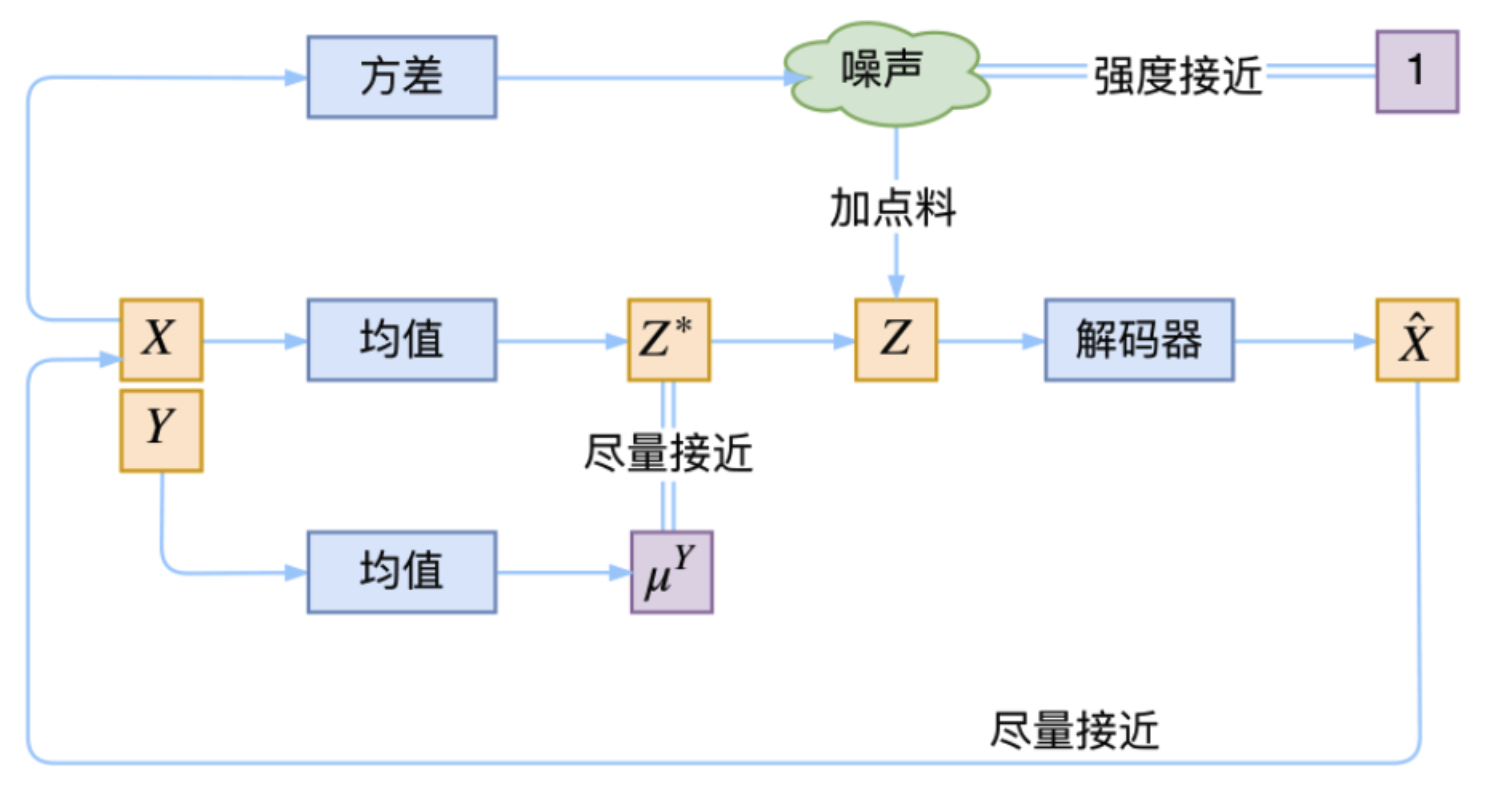
\includegraphics[width=\textwidth]{figures/chapter2/cond_vae.png}
    \caption{条件VAE}
    \label{fig:cond_vae}
\end{figure}
本质分析完了,看贝叶斯派是如何通过理论推导出这么精妙的算法的?

\subsection{VAE的理论推导}
\paragraph{首先声明一些定义}
出发点没变。首先我们有一批数据样本 ${x1,…,xn}$,其整体用$x$来描述,我们希望借助隐变量$z$描述$x$的分布$\hat{p}(x)$,这样(理论上)我们既描述了,$\hat{p}(x)$又得到了生成模型$p(x|z)$,一举两得。
\begin{quotation}
    在贝叶斯框架中,三个核心概念是先验分布、后验分布和似然函数。
    \begin{itemize}
        \item 先验分布$\theta$是在考虑任何观察数据之前,对未知参数$\theta$的概率分布的初始估计。
        \item 似然函数$p(x|z)$描述了给定参数$\theta$的情况下,观测到特定数据x的可能性。
        \item 后验分布$p(z|x)$是在观察到数据$x$之后,对参数$\theta$的概率分布的更新。
    \end{itemize}
\end{quotation}
隐变量$z$在这里对应先验分布,因为在生成这个任务中,我们并没有看到数据x的分布,z只是x的一个初始估计。
而decoder对应似然函数$p(x|z)$,对于一个先验分布z,对z进行映射,得到目标分布p(x)。
encoder则对应后验分布$p(z|x)$,对于真实的数据分布x,对先验分布进行更新。

我们希望得到很好的尽量接近真实的后验分布,使得encoder能够提取出真实数据的有效特征。
因此我们希望最小化encoder的分布和真实后验分布之间的距离,使用KL散度
\begin{align}
    & KL\left(q_\phi\left(z\mid\boldsymbol{x}\right)||p\left(z\mid\boldsymbol{x}\right)\right) \\
    =&\int_zq_\phi\left(z\mid\boldsymbol{x}\right)\log\left[\frac{q_\phi\left(z\mid\boldsymbol{x}\right)}{p\left(z\mid\boldsymbol{x}\right)}\right]dz \\
    =&\int_zq_\phi\left(z\mid\boldsymbol{x}\right)\log\left[\frac{q_\phi\left(z\mid\boldsymbol{x}\right)p(\boldsymbol{x})}{p\left(z,\boldsymbol{x}\right)}\right]dz \\
    =&\int_zq_\phi\left(z\mid\boldsymbol{x}\right)\mathrm{log}\left[\frac{q_\phi\left(z\mid\boldsymbol{x}\right)}{p\left(z,\boldsymbol{x}\right)}\right]dz\boldsymbol{+}\int_zq_\phi\left(z\mid\boldsymbol{x}\right)\mathrm{log}p\left(\boldsymbol{x}\right)dz \\
    =&\mathbb{E}_{q_\phi(z\mid\boldsymbol{x})}\mathrm{log}{\left[\frac{q_\phi\left(z\mid\boldsymbol{x}\right)}{p\left(z,\boldsymbol{x}\right)}\right]}+\mathrm{log}p\left(\boldsymbol{x}\right)
\end{align}
因此得到
\begin{equation}
    KL\left(q_\phi\left(z\mid x\right)||p\left(z\mid x\right)\right)+\mathbb{E}_{q_\phi\left(z\mid\boldsymbol{x}\right)}\mathrm{log}\left[\frac{p\left(z,\boldsymbol{x}\right)}{q_\phi\left(z\mid\boldsymbol{x}\right)}\right]=\mathrm{log}p\left(\boldsymbol{x}\right)
\end{equation}
这个期望项被称为ELBO(Evidence Lower Bound)证据下界

因为真实分布$p(x)$是已知的,所以可以发现,为了让KL散度的项尽可能小,也就是让ELBO尽可能大, 如图\ref{fig:elbo}。
\begin{figure}[htbp]
    \centering
    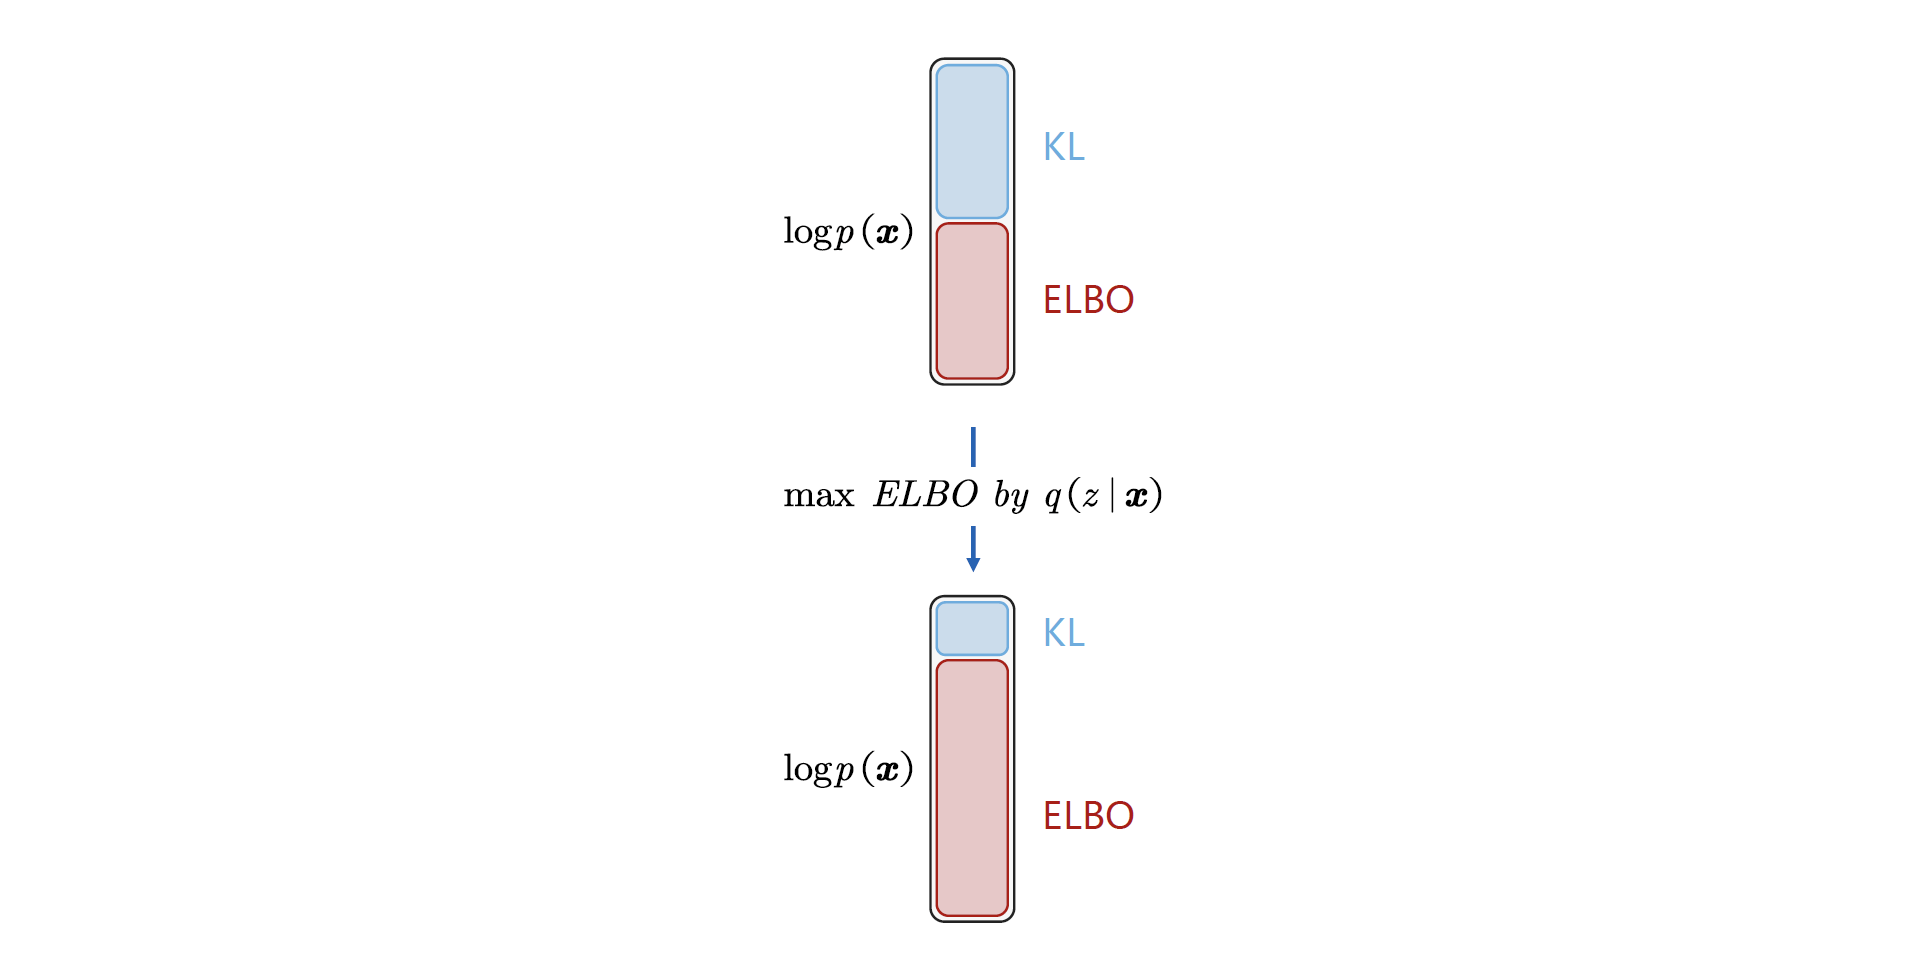
\includegraphics[width=\textwidth]{figures/chapter2/elbo.png}
    \caption{ELBO}
    \label{fig:elbo}
\end{figure}
\begin{align}
 & \mathbb{E}_{q_\phi(z\mid\boldsymbol{x})}\mathrm{log}{\left[\frac{p(z,\boldsymbol{x})}{q_\phi(z\mid\boldsymbol{x})}\right]} \\
 & =\mathbb{E}_{q_\phi(z\mid\boldsymbol{x})}{\left[\log\frac{p_\theta\left(\boldsymbol{x}\mid z\right)p(z)}{q_\phi\left(z\mid\boldsymbol{x}\right)}\right]}\quad \\
 & =\mathbb{E}_{q_\phi(z\mid\boldsymbol{x})}[\mathrm{log}p_\theta(\boldsymbol{x}\mid z)]+\mathbb{E}_{q_\phi(z\mid\boldsymbol{x})}[\mathrm{log}\frac{p(z)}{q_\phi(z\mid\boldsymbol{x})}] \\
 & =\mathbb{E}_{q_\phi(z\mid\boldsymbol{x})}[\log p_\theta(\boldsymbol{x}\mid z)]-KL\left(q_\phi(z\mid\boldsymbol{x})\|p\left(z\right)\right) 
 \label{eq:elbo}
\end{align}
其中式\ref{eq:elbo}的左半边式对应
\begin{equation}
    ||x-\hat{x}||^2
\end{equation}
是MSE重构损失;
右半边式对应
\begin{equation}
    \frac{1}{2}\left( \mu_\phi + \sigma_\phi^2 - 1 - \log(\sigma_\phi^2) \right)
\end{equation}
是KL散度,表示潜在空间分布和标准正态分布的差异。

上面的期望项可以理解为对于每一个后验,我都希望似然函数越大越好,也就是重建的可能越大越好,这个可以理解为希望生成样本和真实样本越接近越好,可以用负的MSE来表示这个重建项,也就是在式子中我们希望期望项越大越好,等价于在MSE中我们希望越小越好。
这里同样(和\ref{sec:vae_essence}对比理解)为了防止方差为0,(方差为0就上式就是无穷大了),我们固定后验为一个标准高斯分布(理由上面描述的已经很充分了)

\begin{figure}[htbp]
    \centering
    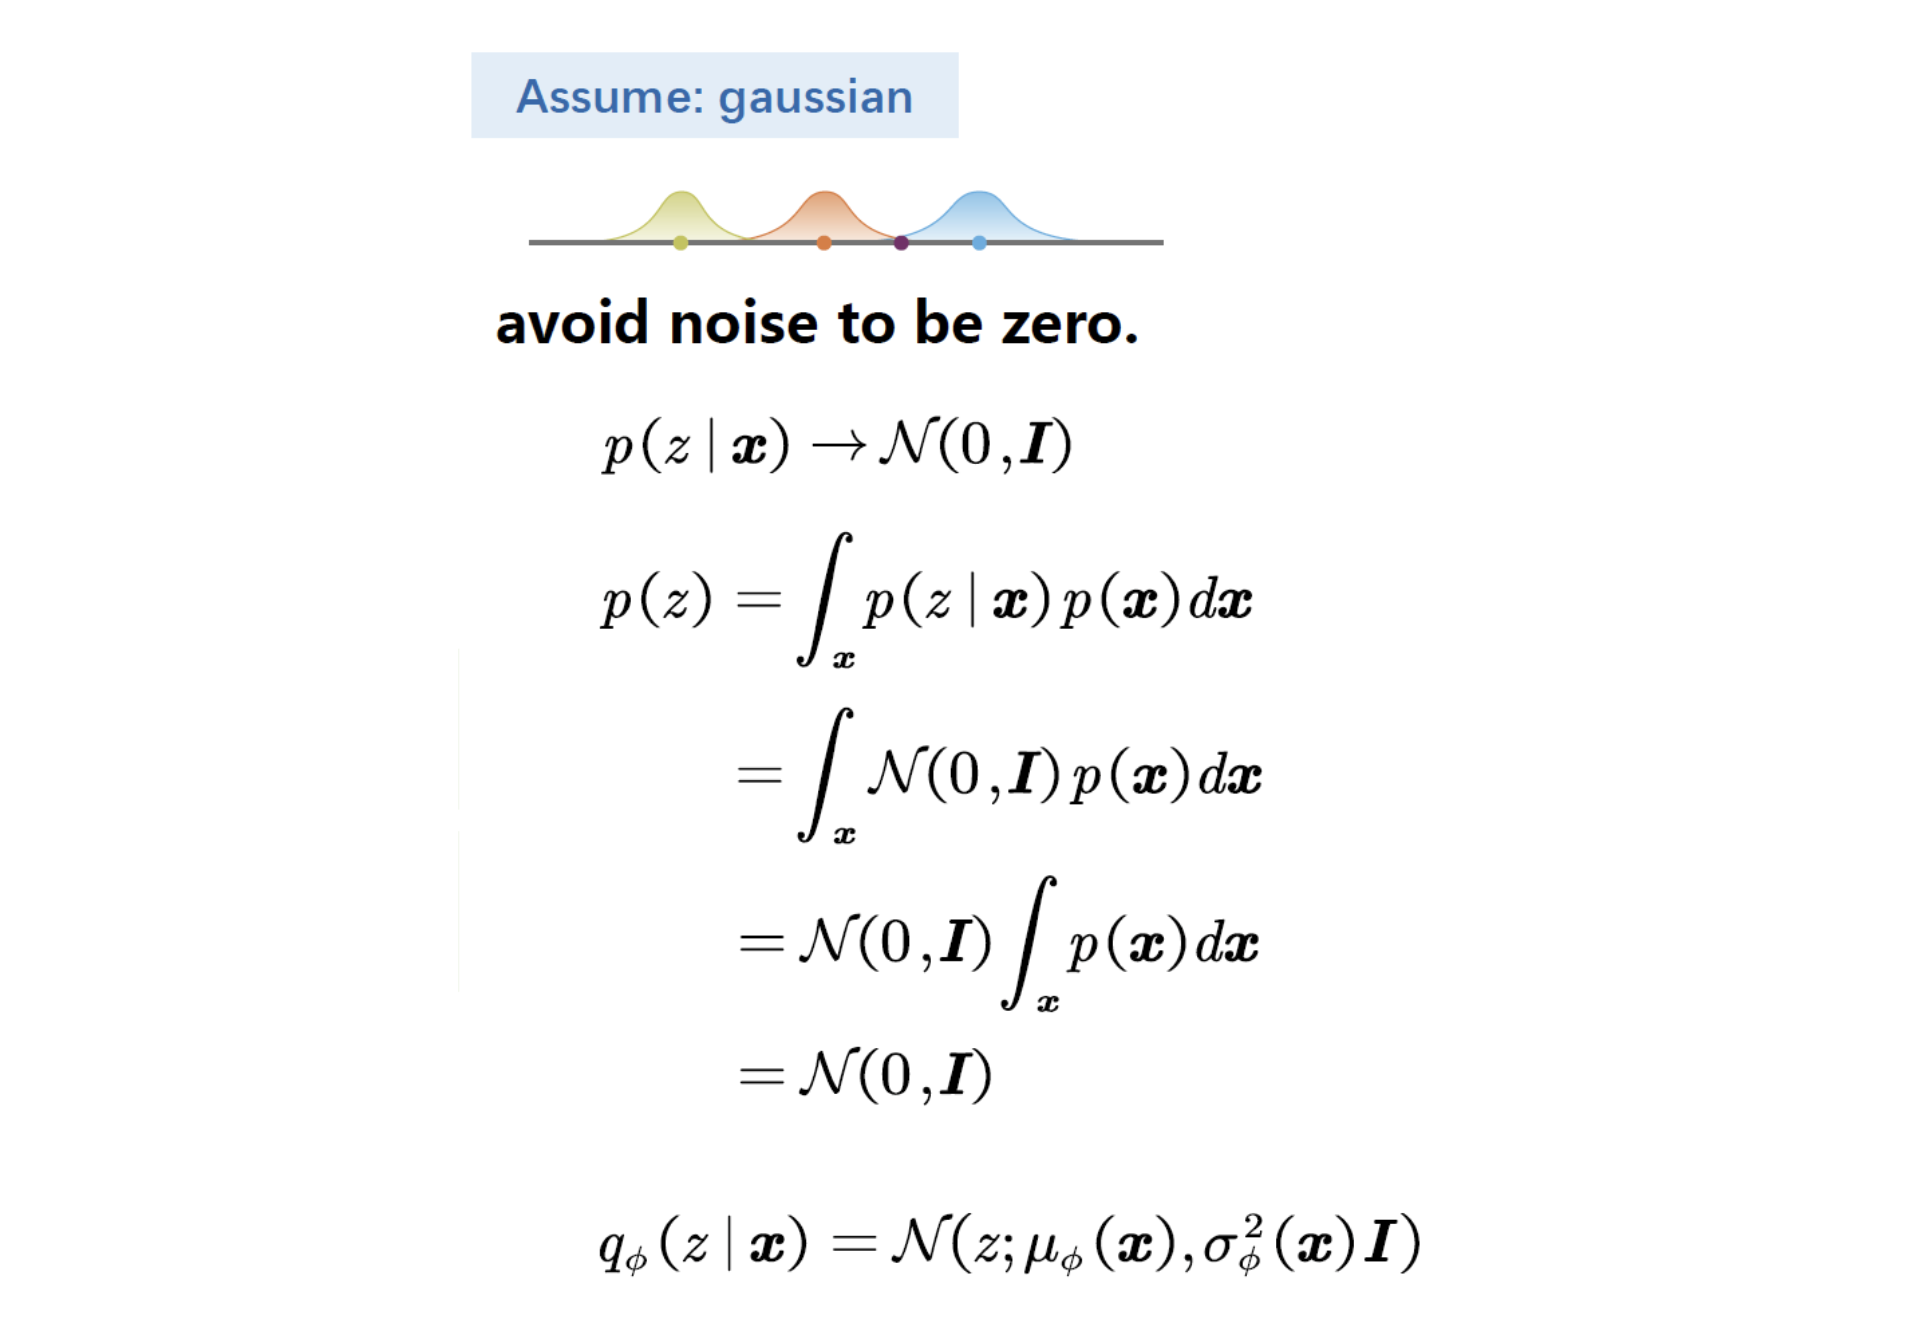
\includegraphics[width=\textwidth]{figures/chapter2/assum.png}
    \caption{潜在空间分布}
    \label{fig:vae_assumption}
\end{figure}
这样我们就得到了和\ref{sec:vae_essence}一样的结论

其中重构项$||\boldsymbol{x} - \hat{\boldsymbol{x}}||^2$对应着真实样本和生成样本的靠近,对应式子中的期望项当然越大越好;后验匹配项$\frac{1}{2} (\mu_{\phi} + \sigma_{\phi}^2 - log \sigma_{\phi}^2 - 1)$对应着后验和标准正态分布的距离,当然越小越好。
这样ELBO越大越好和\ref{sec:vae_essence}就完美吻合了。

\begin{figure}[htbp]
    \centering
    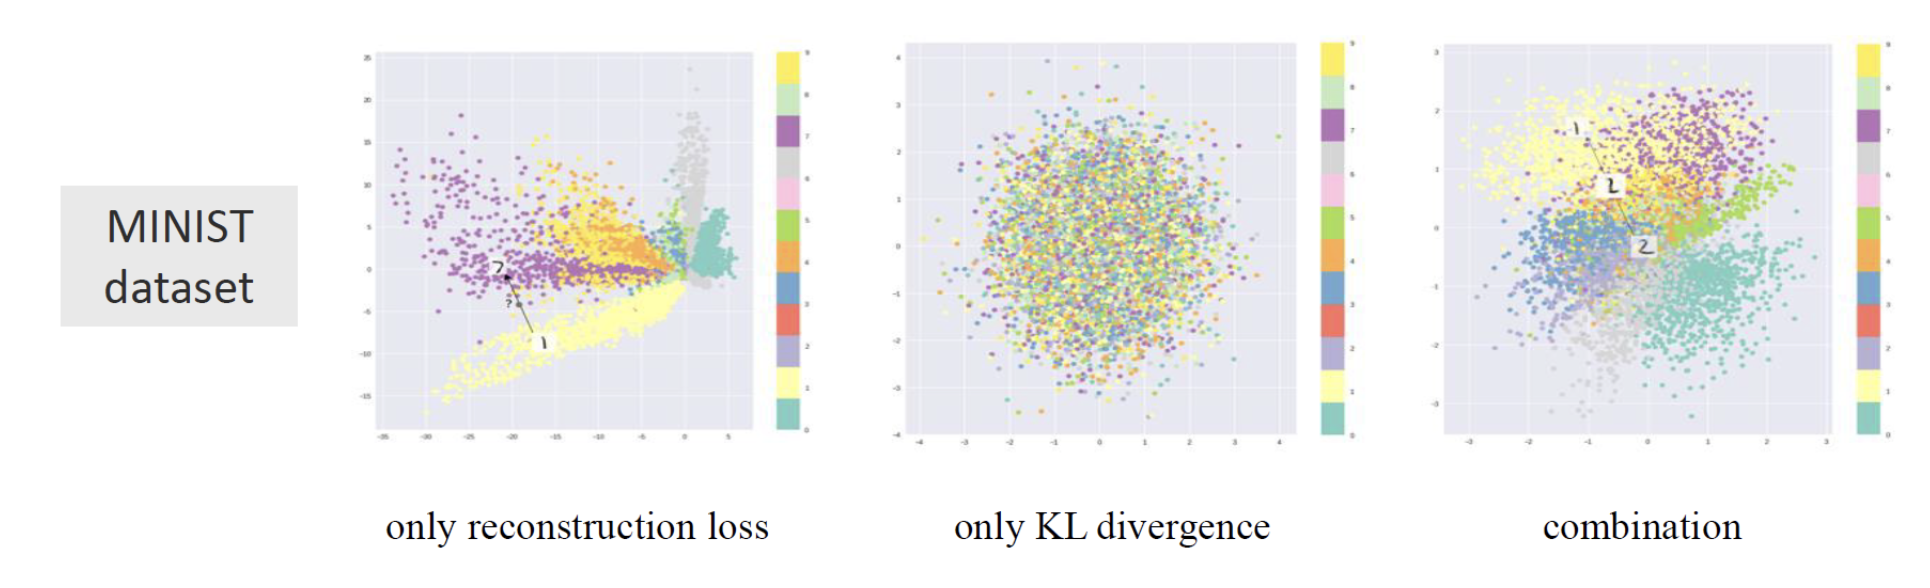
\includegraphics[width=0.9\textwidth]{figures/chapter2/data.png}
    \caption{minist数据集上的数据分布}
    \label{fig:vae_data}
\end{figure}
如图\ref{fig:vae_data},可以看在minist数据集上的测试结果。
\begin{itemize}
    \item 第一张图对应不对隐变量分布进行干涉的结果;\textbf{类别之间差距过大且不连续(退化成AE)}
    \item 第二张图对应不考虑真实样本和生成样本靠近的结果;\textbf{得不到结果}
    \item 第三张图对应两个都考虑的结果;\textbf{类别连续平滑,分布密集}
\end{itemize}

\subsection{局限性}
两个Loss分别展现了局限性
\begin{enumerate}
    \item 对于KL Loss,后验分布和先验分布是不完全相等的
        \begin{itemize}
            \item 信息丢失:这意味着解码器在将数据压缩到潜在空间时丢失信息
            \item 潜在空间结构:可能意味着潜在空间不规则,不连续
        \end{itemize}
        \textbf{解决方案:LDM}
    \item 对于MSELoss,本身可能会趋于让图片更加模糊
        \begin{itemize}
            \item 平均效应:逐像素的最小化导致模型倾向生成一个“平均”的结果
            \item 噪声敏感性:为了最小化这些噪声的影响,模型可能会生成一个更加平滑的结果
        \end{itemize}
        \textbf{解决办法:对抗损失(GAN)}
\end{enumerate}

\begin{figure}[htbp]
    \centering
    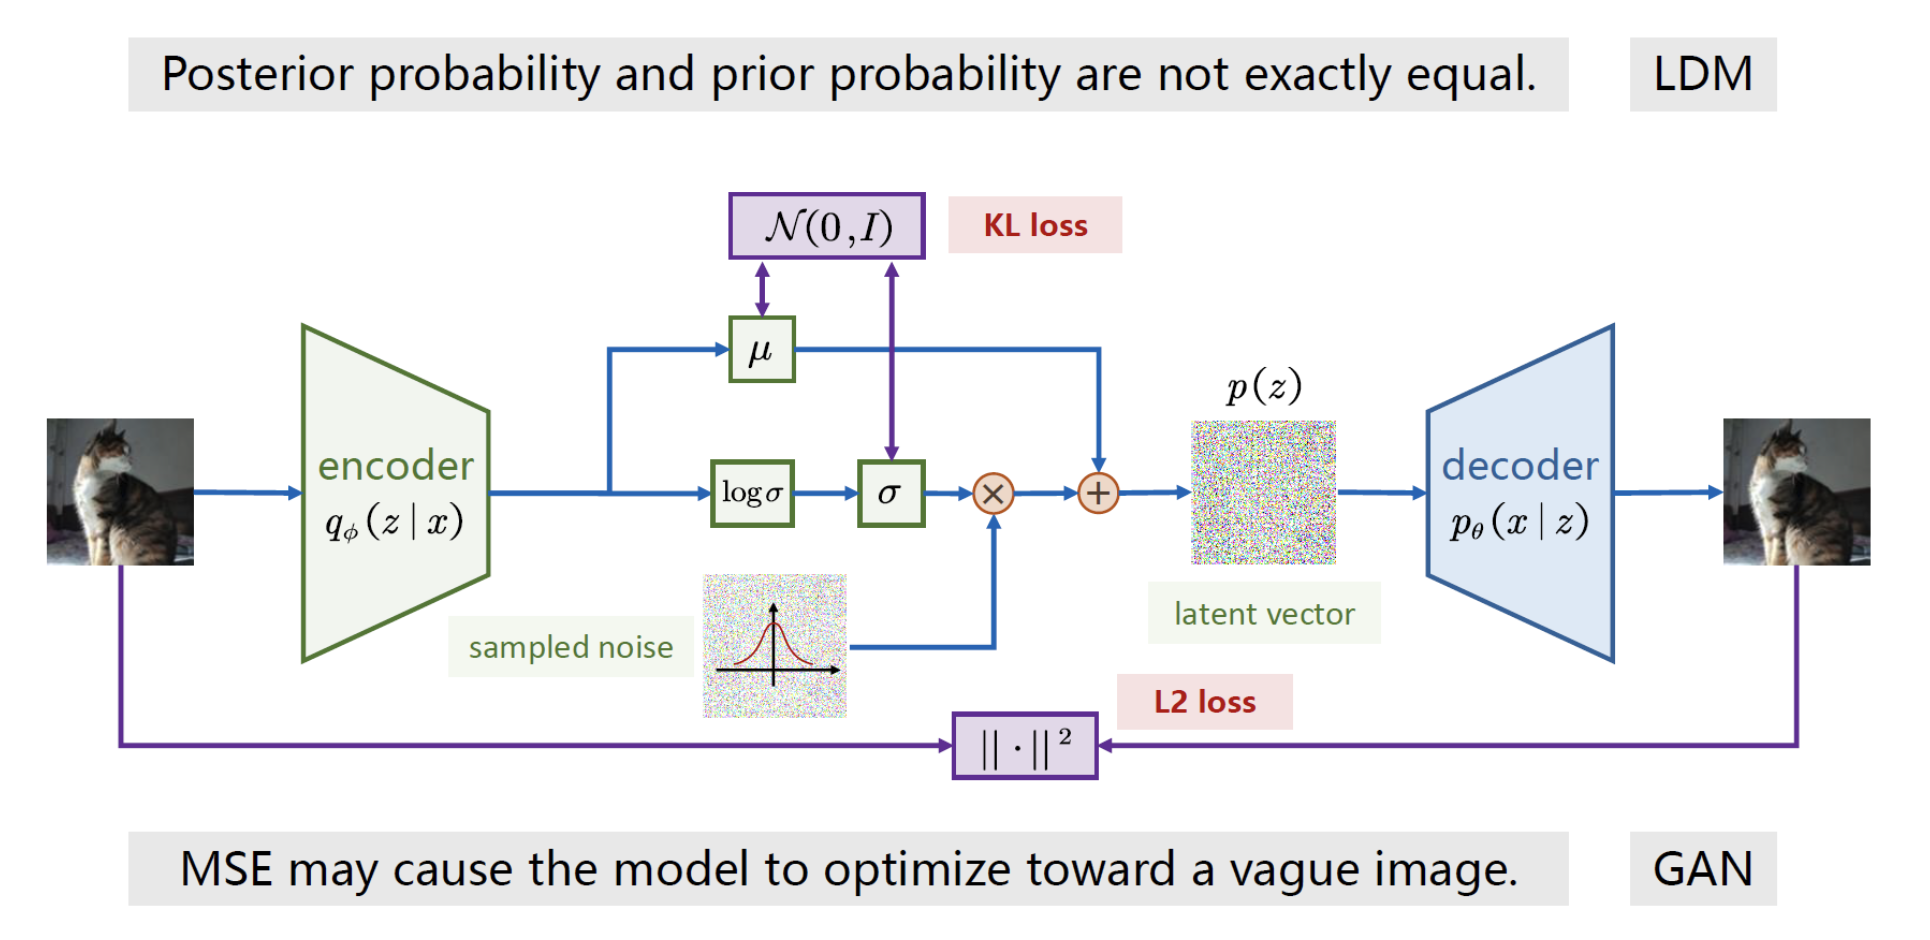
\includegraphics[width=\textwidth]{figures/chapter2/shortcoming.png}
    \caption{VAE的局限性}
    \label{fig:vae_limit}
\end{figure}

\FloatBarrier


\section{参考文献}
\begin{enumerate}
    \item Kingma D P, Welling M. Autoencoding variational bayes. arXiv, 2013.
    \item Understanding Variational Autoencoders (VAEs)
    \item https://spaces.ac.cn/archives/5253 (苏剑林 , 变分自编码器(一):原来是这么一回事)
    \item https://kexue.fm/archives/5343(苏剑林 , 变分自编码器(二):从贝叶斯观点出发)
    \item https://www.bilibili.com/video/BV1ix4y1x7MR/(吃花椒的麦【大白话02】一文理清 VAE 变分自编码器 | 原理图解+公式推导)
\end{enumerate}




